\section{Methodology}

\subsection{Model architecture}

% insert picture Architecture.png
\begin{figure}[h]
    \centering
    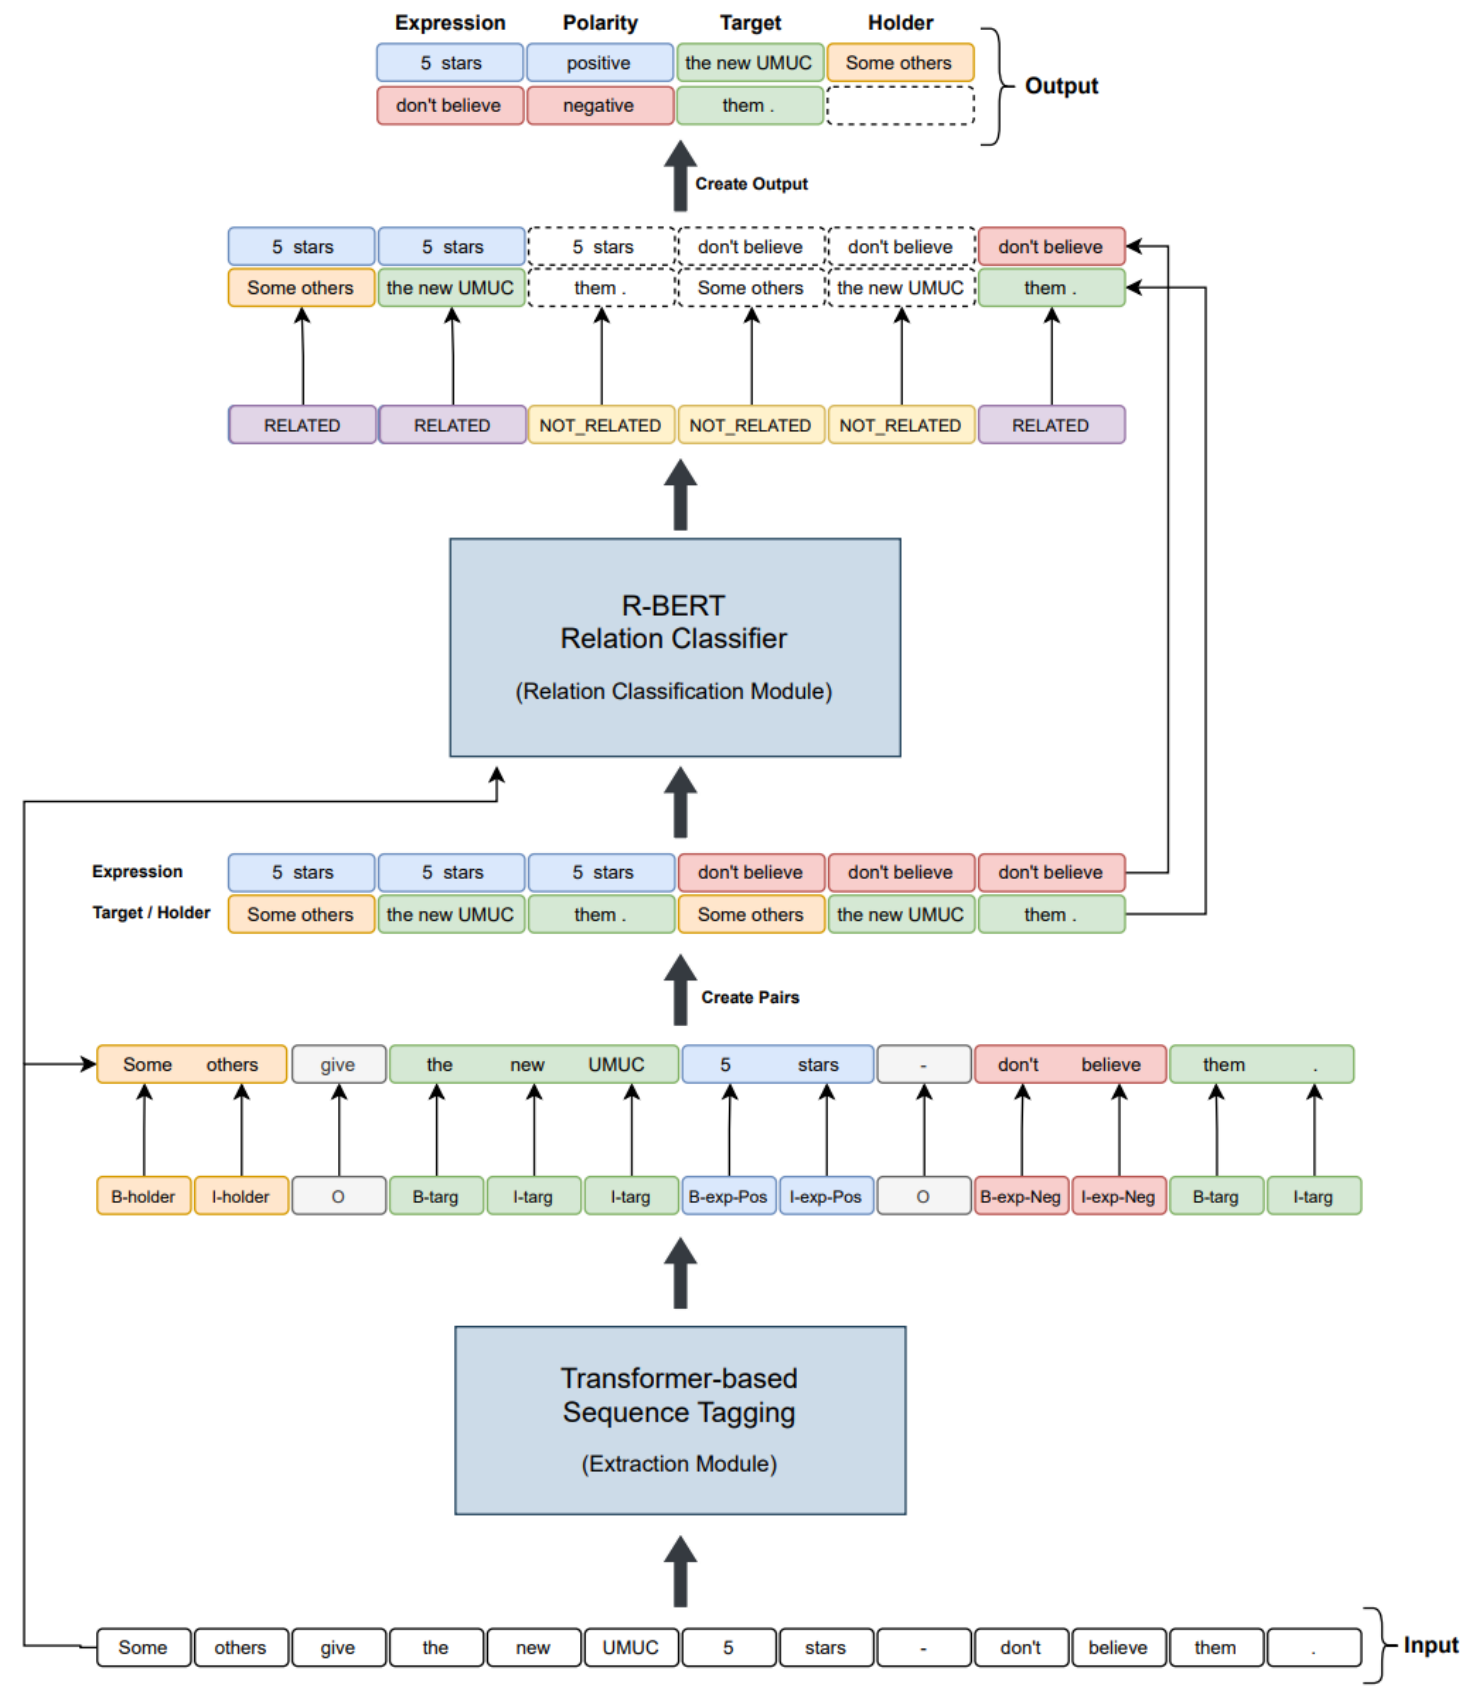
\includegraphics[width=0.8\textwidth]{Architecture.png}
    \caption{Model architecture}
    \label{fig:Architecture}
\end{figure}

The methodology used in this project involved leveraging the SKEP model for both opinion extraction and relation classification tasks. Specifically, we utilized a sequence labeling approach for opinion extraction, where each token in the input text is classified as either an attribute, an opinion word, or a non-relevant token. We then concatenated the identified attributes and opinion words to form opinion pairs, which we used to classify the sentiment polarity of each attribute.

For relation classification, we concatenated each opinion pair with the original text and fed it into the SKEP model, which predicted the sentiment polarity of each attribute. We fine-tuned the SKEP model on our labeled dataset using a supervised learning approach, optimizing the model hyperparameters for the best performance.

The model hyperparameters we used for both opinion extraction and relation classification were set as follows: num epoch = 3, learning rate = 3e-5, weight decay = 0.01, warmup proportion = 0.1, max grad norm = 1.0, log step = 20, eval step = 100, and seed = 1000. We selected these hyperparameters based on prior research and empirical testing, aiming to achieve a balance between model performance and training efficiency.

Figure \ref{fig:Architecture} shows the model architecture. \cite{poswiata-2022-opi}

\subsection{Evaluation and Output}

We used the F1 score as our primary evaluation metric and experimented with different model architectures and hyperparameters to achieve optimal performance. Specifically, we used the BIO tagging scheme for opinion extraction and fine-tuned the SKEP model for relation classification.